\begin{exercise}
      {ID-b8804547d0d591c4238b208f8f21c16a66d5bf64}
      {Zugfahrt}
  \ifproblem\problem\par
    % <PROBLEM>
    Eine historische Eisenbahn befährt eine Kurzstrecke.
    Dabei übernimmt zur Entlastung des Fahrers ein Computer
    die Geschwindigkeitssteuerung. Er ist so programmiert,
    dass der zurückgelegte Weg durch eine ganzrationale
    Funktion $s$ mit
    \begin{equation*}
      s(t)=at^3+bt^2+ct+d
      \qquad\text{($t$ in \si{\minute}, $s(t)$ in \si{\kilo\metre})}
    \end{equation*}
    beschrieben werden kann.
    Ein aufmerksamer Fahrgast stellt fest, dass
    die gesamte Fahrt 8 Minuten dauert. Außerdem
    beobachtet er, dass nach 4 Minuten Fahrt
    \SI{4}{\kilo\metre} zurückhelegt werden.
    Am Anfang und am Ende der Fahrt steht der Zug.
    \par
    Bestimmen Sie die Gleichung der
    Weg-Zeit-Funktion $s$.
    \par
    \textit{Hinweis:} Die Geschwindigkeit $v$ ist
    die Ableitung des Weges $s$.
    % </PROBLEM>
  \fi
  \ifoutline\outline\par
    % <OUTLINE>
    Folgende Informationen sind in der
    Aufgabenstellung vorhanden:
    \begin{enumerate}[a)]
      \item $s(t)$ beschreibt den zurückgelegten Weg
      \item nach 4 Minuten hat der Zug
            \SI{4}{\kilo\metre} zurückgelegt
      \item die Geschwindigkeit ist die Ableitung des Weges
      \item am Anfang der Fahrt steht der Zug
      \item am Ende der Fahrt (die Fahrt dauert
            8 Minuten) steht der Zug
    \end{enumerate}
    % </OUTLINE>
  \fi
  \ifoutcome\outcome\par
    % <OUTCOME>
    Aus den Informationen der Aufgabenstellung
    lassen sich folgende Gleichungen ableiten:
    \begin{enumerate}[a)]
      \item $s(t)=at^3+bt^2+ct+d$ beschreibt den
            zurückgelegten Weg:
            \begin{equation*}
              s(0)=0
              \quad\Rightarrow\quad
              d=0
            \end{equation*}
      \item nach 4 Minuten hat der Zug
            \SI{4}{\kilo\metre} zurückgelegt:
            \begin{equation*}
              s(4)=4
            \end{equation*}
      \item die Geschwindigkeit ist die Ableitung des Weges
            \begin{equation*}
              v(t)=s'(t)=3at^2+2bt+c
            \end{equation*}
      \item am Anfang der Fahrt steht der Zug:
            \begin{equation*}
              s'(0)=0
              \quad\Rightarrow\quad
              c=0
            \end{equation*}
      \item am Ende der Fahrt (die Fahrt dauert
            8 Minuten) steht der Zug:
            \begin{equation*}
              s'(8)=0
            \end{equation*}
    \end{enumerate}
    Die gesuchste Funktion und deren erste Ableitung
    haben also folgende vorläufige Form:
    \begin{equation*}
      s(t)=at^3+bt^2
      \quad\text{und}\quad
      s'(t)=3at^2+2bt
    \end{equation*}
    Die noch unbekannten Koeffizienten $a$ und
    $b$ ergeben sich dann aus folgendem
    Gleichungssystem:
    \begin{equation*}
      \setlength{\arraycolsep}{0.1em}%
      \begin{array}{r|lcr}
         \text{I}\;\; & \;  s(4) & = & 4 \\
        \text{II}\;\; & \; s'(8) & = & 0
      \end{array}
      \quad\Rightarrow\quad
      %s(t)=at^3+bt^2
      %s'(t)=3at^2+2bt
      \begin{array}{r|rcrcr}
         \text{I}\;\; & \;  a\cdot4^3 & + &  b\cdot4^2 & = & 4 \\
        \text{II}\;\; & \; 3a\cdot8^2 & + & 2b\cdot8   & = & 0
      \end{array}
    \end{equation*}
    \par Als Lösung erhält man:\\
    \begin{minipage}[t]{0.49\linewidth}
      \vspace*{-\abovedisplayskip}
      \begin{alignat*}{1}
        % <STEP>
        &\setlength{\arraycolsep}{0.1em}%
        \begin{array}{r|rrrrrrrl}
         \text{I}{\,} & {\,} &  \num{64}a & + & \num{16}b & = & \num{4} & {\quad} & |:\num{4}  \\
        \text{II}{\,} & {\,} & \num{192}a & + & \num{16}b & = & \num{0} & {\quad} & |:\num{16}
        \end{array}
        % </STEP>
        % <STEP>
        \\[1ex]&\setlength{\arraycolsep}{0.1em}%
        \begin{array}{r|rrrrrrrl}
         \text{I}{\,} & {\,} & \num{16}a & + & \num{4}b & = & \num{1} & {\quad} &                                    \\
        \text{II}{\,} & {\,} & \num{12}a & + & \num{1}b & = & \num{0} & {\quad} & |\cdot\num{4}-\num{3}\cdot\text{I}
        \end{array}
        % </STEP>
      \end{alignat*}
    \end{minipage}%
    \hfill
    \begin{minipage}[t]{0.49\linewidth}
      \vspace*{-\abovedisplayskip}
      \begin{alignat*}{1}
        % <STEP>
        &\setlength{\arraycolsep}{0.1em}%
        \begin{array}{r|rrrrrrrl}
         \text{I}{\,} & {\,} & \num{16}a & + & \num{4}b & = &  \num{1} & {\quad} & |\cdot\num{2}+\text{II}     \\
        \text{II}{\,} & {\,} &  \num{0}a & - & \num{8}b & = & -\num{3} & {\quad} & |\cdot\left(-\num{1}\right)
        \end{array}
        % </STEP>
        % <STEP>
        \\[1ex]&\setlength{\arraycolsep}{0.1em}%
        \begin{array}{r|rrrrrrrl}
         \text{I}{\,} & {\,} & \num{32}a & + & \num{0}b & = & -\num{1} & {\quad} &   \\
        \text{II}{\,} & {\,} &  \num{0}a & + & \num{8}b & = &  \num{3} & {\quad} &
        \end{array}
        % </STEP>
      \end{alignat*}
    \end{minipage}\par
    Der gesuchte Funktionsterm lautet also:
    \begin{equation*}
      %<OCTAVE>
      s(t)=-\frac{\num{1}}{\num{32}}t^{3}+\frac{\num{3}}{\num{8}}t^{2}
      %</OCTAVE>
      %s = [-1/32 3/8 0 0];
      %printf("s(t)=%s\n", mypolystr(s, "t", [0,0,0,0,1]));
    \end{equation*}
    \begin{center}
      %<OCTAVE>
      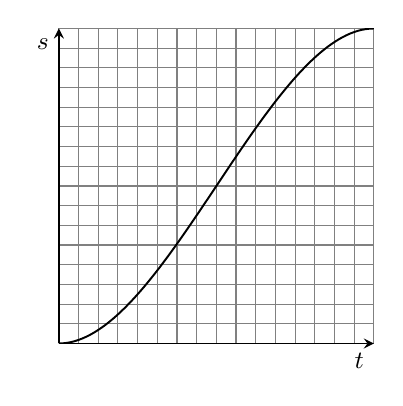
\begin{tikzpicture}[scale=0.500]
        % grid
        \draw[draw=black!50!white] (0.000, 0.000) grid[step=0.5] (8.000, 8.000);
        % x-axis
        \draw[line width=0.6pt, ->, >=stealth] (0.000, 0) -- (8.000, 0) node[below left] {\small$t$};
        % y-axis
        \draw[line width=0.6pt, ->, >=stealth] (0, 0.000) -- (0, 8.000) node[below left] {\small$s$};
        % function: f(x)=-\num{0.03125}x^{3}+\num{0.375}x^{2}
        \begin{scope}[line width=0.7pt]
          \clip (0.000, 0.000) rectangle (8.000, 8.000);
          \draw plot[smooth] coordinates
          {
            (  0.000,   0.000) (  0.100,   0.004) (  0.200,   0.015)
            (  0.300,   0.033) (  0.400,   0.058) (  0.500,   0.090)
            (  0.600,   0.128) (  0.700,   0.173) (  0.800,   0.224)
            (  0.900,   0.281) (  1.000,   0.344) (  1.100,   0.412)
            (  1.200,   0.486) (  1.300,   0.565) (  1.400,   0.649)
            (  1.500,   0.738) (  1.600,   0.832) (  1.700,   0.930)
            (  1.800,   1.033) (  1.900,   1.139) (  2.000,   1.250)
            (  2.100,   1.364) (  2.200,   1.482) (  2.300,   1.604)
            (  2.400,   1.728) (  2.500,   1.855) (  2.600,   1.986)
            (  2.700,   2.119) (  2.800,   2.254) (  2.900,   2.392)
            (  3.000,   2.531) (  3.100,   2.673) (  3.200,   2.816)
            (  3.300,   2.961) (  3.400,   3.107) (  3.500,   3.254)
            (  3.600,   3.402) (  3.700,   3.551) (  3.800,   3.700)
            (  3.900,   3.850) (  4.000,   4.000) (  4.100,   4.150)
            (  4.200,   4.300) (  4.300,   4.449) (  4.400,   4.598)
            (  4.500,   4.746) (  4.600,   4.893) (  4.700,   5.039)
            (  4.800,   5.184) (  4.900,   5.327) (  5.000,   5.469)
            (  5.100,   5.608) (  5.200,   5.746) (  5.300,   5.881)
            (  5.400,   6.014) (  5.500,   6.145) (  5.600,   6.272)
            (  5.700,   6.396) (  5.800,   6.518) (  5.900,   6.636)
            (  6.000,   6.750) (  6.100,   6.861) (  6.200,   6.967)
            (  6.300,   7.070) (  6.400,   7.168) (  6.500,   7.262)
            (  6.600,   7.351) (  6.700,   7.435) (  6.800,   7.514)
            (  6.900,   7.588) (  7.000,   7.656) (  7.100,   7.719)
            (  7.200,   7.776) (  7.300,   7.827) (  7.400,   7.872)
            (  7.500,   7.910) (  7.600,   7.942) (  7.700,   7.967)
            (  7.800,   7.985) (  7.900,   7.996) (  8.000,   8.000)
          };
        \end{scope}
      \end{tikzpicture}
      %</OCTAVE>
      %s = [-1/32 3/8 0 0];
      %mypolyplot(s, 0, 8, 0, 8, 0.1);
    \end{center}
    % </OUTCOME>
  \fi
\end{exercise}
